\chapter{Impedance Control for Centric Motion}
%%%%%%%%%%%%%%%%%%%%%%%%%%%%%%%%%%%%%%%%%%%%%%%%%%%%%%%%%%%%%%%%%%%%%%%%%%%%%%%%

In this chapter, we will introduce the fundamental concept of impedance control and how can we achieve it in the multi-link aerial robots, as well as a new insight of impedance control. After that, the special setting on the 2D mutli-link aerial robot Hydrus Xi and on the 3D multi-link aerial robot Dragon will be introduced. Finally, due to some tasks need to select the impedance acting coordinate, we will introduce the task-oriented impedance coordinate selection method.
% We will discuss a new concept of impedance controller.
% also what should we consider when choosing the parameters in impedance and admittance controller
% \section{Motivation}

% The motivation for this hybrid impedance-admittance control framework is to provide both resilience and adaptivity when sliding on an unknown surface, where geometry and friction introduce significant uncertainties.

%%%%%%%%%%%%%%%%%%%%%%%%%%%%%%%%%%%%%%%%%%%%%%%%%%%%%%%%%%%%%%%%%%%%%%%%%%%%%%%%



%%%%%%%%%%%%%%%%%%%%%%%%%%%%%%%%%%%%%%%%%%%%%%%%%%%%%%%%%%%%%%%%%%%%%%%%%%%%%%%%
\section{Impedance Control Normal setup}

% In this section, we will introduce how to adjust parameters to make the aerial robot to meet the require performance.
% In this subsection, we will introduce the 
Impedance control models the robot as a second-order system in the sight of environment, so that the robot can adjusting its own movement by external force \cite{hogan_1984_impedance}. To meat different requirements, the dynamic parameters can be freely designed to achieve the desired interaction behavior. For example, by adjusting the stiffness parameters, the robot can be made resilient in certain directions to reject disturbances while remaining compliant in others to maintain safe interaction \cite{bodie_2020_active}. In this section, we will introduce how to get the command wrench equation of impedance control.

We will obtain the motion by translational and rotational, seperatively. The translational motion is expressed in the world frame $\{W\}$, whereas the rotational motion is expressed in the CoG frame $\{C\}$. Under this convention, the impedance equations are written as:
\begin{subequations}
\label{eq:impedance control 1}
\begin{align}
    {\boldsymbol{M}_{d}}{^W\!\ddot{\boldsymbol{p}}}+{\boldsymbol{C}_{td}}{\boldsymbol{e}_v}+{\boldsymbol{K}_{td}}{\boldsymbol{e}_p}&={^W\!\boldsymbol{\tilde{f}}_{ext}}, \\[2pt]
    {\boldsymbol{I}_{d}}{^C\!\dot{\boldsymbol{\omega}}}+{\boldsymbol{C}_{rd}}{\boldsymbol{e}_\omega}+{\boldsymbol{K}_{rd}}{\boldsymbol{e}_R}&={^C\!\boldsymbol{\tilde{\tau}}_{ext}},
\end{align}
\end{subequations}
where ${\boldsymbol{M}_{d}}\in \mathbb{R}^{3\times3}$ is the desired virtual mass, ${\boldsymbol{I}_{d}}\in \mathbb{R}^{3\times3}$ is the desired virtual inertia, ${\boldsymbol{C}_{td}}\in \mathbb{R}^{3\times3}$, ${\boldsymbol{C}_{rd}}\in \mathbb{R}^{3\times3}$ are the desired linear and rotational damping matrices, and ${\boldsymbol{K}_{td}}\in \mathbb{R}^{3\times3}$, ${\boldsymbol{K}_{rd}}\in \mathbb{R}^{3\times3}$ are the desired linear and rotational stiffness matrices, respectively. All of these matrices are positive definite. These are what we want the system performs like. Here the error vectors in (\ref{eq:impedance control 1}) are defined as:
\begin{subequations}
\label{eq:error of rotation}
\begin{align}
    {\boldsymbol{e}_p}&={^W\!\boldsymbol{p}}-{^W\!\boldsymbol{p}_{ref}}, \\[2pt]
    {\boldsymbol{e}_v}&={^W\!\dot{\boldsymbol{p}}}-{^W\!\dot{\boldsymbol{p}}_{ref}}, \\[2pt]
    {\boldsymbol{e}_R}&=\frac{1}{2}({^W\!\boldsymbol{R}^{\mathrm{T}}_{C,ref}}{^W\!\boldsymbol{R}_{C}}-{^W\!\boldsymbol{R}^{\mathrm{T}}_{C}}{^W\!\boldsymbol{R}_{C,ref}})^\vee, \\[2pt]
    {\boldsymbol{e}_\omega}&={^C\!\boldsymbol{\omega}}-{^W\!\boldsymbol{R}^{\mathrm{T}}_{C}}{^W\!\boldsymbol{\omega}}_{ref},
\end{align}
\end{subequations}
where we use the vee-operator $^\vee$ to extract a vector from a skew symmetric matrix.

Next, by substituting the dynamic equations \eqref{eq:dynamics} into the impedance control equations \eqref{eq:impedance control 1} in order to eliminate $\ddot{\boldsymbol{p}}$ and $\dot{\boldsymbol{\omega}}$, the command wrench added on the CoG can be derived. The translational component can be written as

\begin{equation}
\label{eq:imp cmd for trans1}
    {^W\!\boldsymbol{f}_{cmd}}=(m\boldsymbol{M}^{-1}_d-\boldsymbol{E}_3){^W\!\boldsymbol{\tilde{f}}_{ext}}-m\boldsymbol{M}_d^{-1}({\boldsymbol{C}_{td}}{\boldsymbol{e}_v}+{\boldsymbol{K}_{td}}{\boldsymbol{e}_p})+m\boldsymbol{g}.
\end{equation}

And the rotational component can be written as

\begin{equation}
\label{eq:imp cmd for rot1}
    {^{C}\boldsymbol{\tau}_{cmd}}=(\boldsymbol{I}\boldsymbol{I}^{-1}_d-\boldsymbol{E}_3){^{C}}\boldsymbol{\tilde{\tau}}_{ext}-\boldsymbol{I}\boldsymbol{I}^{-1}_d({\boldsymbol{C}_{rd}}{\boldsymbol{e}_\omega}+{\boldsymbol{K}_{rd}}{\boldsymbol{e}_R})+{^{C}\boldsymbol{\omega}} \times \boldsymbol{I}{^{C}\boldsymbol{\omega}}.
\end{equation}
Here we obtain the command wrench that the rotor of the aerial robot must generate.

Finally, for some reason we will introduce in the next section, we can rewrite the \ref{eq:imp cmd for trans1} and \ref{eq:imp cmd for rot1} as follow.  Here we define the normalized linear damping and stiffness as $\tilde{\boldsymbol{C}}_{td} = \boldsymbol{M}^{-1}_d\boldsymbol{C}_{td}$ and $\tilde{\boldsymbol{K}}_{td} = \boldsymbol{M}^{-1}_d\boldsymbol{K}_{td}$, respectively. Using these definitions, \eqref{eq:imp cmd for trans1} can be rewritten as
\begin{equation}
\label{eq:imp cmd for trans2}
    {^W\!\boldsymbol{f}_{cmd}}=(m\boldsymbol{M}^{-1}_d-\boldsymbol{E}_3){^W\!\boldsymbol{\tilde{f}}_{ext}}-m(\tilde{\boldsymbol{C}}_{td}{\boldsymbol{e}_v}+{\tilde{\boldsymbol{K}}_{td}}{\boldsymbol{e}_p})+m\boldsymbol{g}.
\end{equation}
Also we define the normalized rotation damping and stiffness as $\tilde{\boldsymbol{C}}_{rd} = \boldsymbol{I}^{-1}_d\boldsymbol{C}_{rd}$ and $\tilde{\boldsymbol{K}}_{rd} = \boldsymbol{I}^{-1}_d\boldsymbol{K}_{rd}$, respectively. Equation (\ref{eq:imp cmd for rot1}) can then be rewritten as
\begin{equation}
\label{eq:imp cmd for rot2}
    {^{C}\boldsymbol{\tau}_{cmd}}=(\boldsymbol{I}\boldsymbol{I}^{-1}_d-\boldsymbol{E}_3){^{C}}\boldsymbol{\tilde{\tau}}_{ext}-\boldsymbol{I}(\tilde{\boldsymbol{C}}_{rd}{\boldsymbol{e}_\omega}+\tilde{\boldsymbol{K}}_{rd}{\boldsymbol{e}_\alpha})
    +{^{C}\boldsymbol{\omega}} \times \boldsymbol{I}{^{C}\boldsymbol{\omega}}.
\end{equation}
These equations help generate the command wrench that we want the rotors to perform. In next section, we will explain why we rewrite the equation like these, and will introduce a new insight of impedance control.
% Noting that the normalized matrices are considered as contact parameters and are tuned in free flight situation. This is how we get the command wrench.

%%%%%%%%%%%%%%%%%%%%%%%%%%%%%%%%%%%%%%%%%%%%%%%%%%%%%%%%%%%%%%%%%%%%%%%%%%%%%%%%
\section{Parameter tuning discussion}
One of the most important features of impedance control is the performance of aerial robot can be reshaped due to the specificly designed parameter matrices. However, Tranditional literatures seldomly consider the connection between the parameter selection and the flight and contact behaviours. Even though the parameter matrices usually have specific physical meaning, these physical interpretations do not directly provide a practical parameter selection procedure. Therefore, although the qualitative influence of each parameter is generally understood, determining suitable numerical values remains difficult in practice. 

In this section, by re-analyze the meaning of the impedance parameters, we will obtain a new insight about impedance control, and find the special according relationship between impedance control and PID control. Therefore, the parameters can be better selected according to the resulting system behavior rather than their physical meanings alone. 

% We can find some relationship between PID control and impedance control, therefore use PID inspired tuning method to find the suitable parameters.


Let's consider the following 1-DoF impedance control equation
\begin{equation}
\label{eq:imp cmd analysis1}
  m_d\ddot{p}+c_de_v+k_de_p = f_{ext},
\end{equation}
Here, the parameters $m_d$, $c_d$, $k_d$ are the designed mass, the designed damping, and the designed stiffness, respectively. $\ddot{p}$ is the current acceleration, while $e_v$ and $e_p$ denote the velecity and position error defined as $e_v = \dot{p}-\dot{p}_{ref}$ and $e_p = p-p_{ref}$, respectively. $f_{ext}$ represents the external force.


The dynamic equation of a 1-dof object can be written as
\begin{equation}
\label{eq:imp cmd analysis2}
  m\ddot{p}+g(\dot{p}, p) = f_{ext} + f_{cmd},
\end{equation}
here $g(\dot{p}, p)$ represents an extreme term such as gravity and Coriolis, $f_{cmd}$ is the command force. 
By substituting equation (\ref{eq:imp cmd analysis2}) into equation (\ref{eq:imp cmd analysis1}) in order to  eliminate $\ddot{p}$, we can get

\begin{equation}
\label{eq:imp cmd analysis3}
{{f}_{cmd}}=(\frac{m}{m_d}-1){{f}_{ext}}-m({\frac{c_d}{m_d}e_v+\frac{c_d}{k_d}e_p})+g(\dot{p}, p).
\end{equation}

Theoretically, the three parameters $m_d$, $c_d$ and $k_d$ can be chosen independently refer to the task requirement. 
we define $\tilde{c}_d = \frac{c_d}{m_d}$, $\tilde{k}_d = \frac{k_d}{m_d}$ as the normalized damping and normalized stiffness, respectively. we also use mass ratio $\mu$ to replace $\frac{m}{m_d}$, so the equation becomes 
\begin{equation}
\label{eq:imp cmd analysis4}
{{f}_{cmd}}=(\mu-1){{f}_{ext}}-m({\tilde{c}_de_v+\tilde{k}_de_p})+g(\dot{p}, p).
\end{equation}

If we write the PID control equation as 
\begin{equation}
\label{eq:PID cmd}
{{f}_{cmd}}=-k_pe_p-k_i\int e_p\mathrm{d}t-k_de_v+g(\dot{p}, p).
\end{equation}
Note that the defination of errors here is the current value minus the reference value, therefore here we use minus symbol.

We could find that the two equations are very similar. If we chose $\tilde{c}_d=\frac{k_d}{m}$ and $\tilde{k}_d=\frac{k_p}{m}$, the only differenty lines on the I term $k_i\int e_p\mathrm{d}t$ and the external force  compensation term $(\mu-1){{f}_{ext}}$. Both of them are designed to reduce errors, but the effect is different in the contact situation.

In the context of interaction, due to the contact condition, we may encounter it usually exist persistent position error between the position reference and the contact boundary in the contact direction, or persistent external force related to friction in the moving direction. In the case of contact direction, to reduce the position error, the I term $k_i\int e_p\mathrm{d}t$ will continue integral to increase the command force to infinite except we set a limitation in advance. That is means the integral term unable to respond well to external forces. On the other hand, the external force term $(\mu-1){{f}_{ext}}$ is related to the estimated external force. It can adjust the final command wrench by considering the external force, and the real contact force vary indirectly with changes in position error. In the case of moving direction, the external force term can compensate part of the friction, which means it can perform better than PID control that does not have the imformation of external force. In a word, in the contact scenario, due to consider the external force imformation, the impedance control generally perform better than the PID control.

Considering in other side, the impedance control still has a lot of similarities to the PID control, so we can get some inspiration form PID parameters tuning process. Here we can divide the impedance equation it into PD control part $-m({\frac{c_d}{m_d}e_v+\frac{c_d}{k_d}e_p})$ and external force part $(\frac{m}{m_d}-1){{f}_{ext}}$. If there is no external force, the external force part should disappear, and only PD control part left. So we can use PID turning method to find the parameters $\tilde{c}_d$ and $\tilde{k}_d$, now they are consider as the $k_p$ and $k_d$.

After we tuning the parameters in free flight, it must be consider in contact situation. Let us consider the mass ratio parameter $\mu$. If $\mu$ is set to $0$, the compensation term is exactly the estimated external wrench, so the command will completed compensate the external force. If $\mu$ is set to $1$, the external force term will also disappear, in which situation the impedance controller degenerate to a PD controller. If $\mu > 1$, the external force term has the same direction with the external force, so the command will help to push the aerial robot to the direction of external force, which means the aerial robot will follow the external force. In this situation, the aerial robot can be regarded as compliance, the stiffness is relatively low. On the other hand, if $\mu >1$, the external force term has the reverse direction with the external force, which means the command will help to resist the external force. In this situation, the aerial robot will try to reduce its movement at the direction of external force, the stiffness is relatively high. 

In summary, by setting $\mu$ larger or less than $1$, the aerial robot can perform relatively compliant or rigid. By tuning parameters depend on the task requirements and environment situation, the aerial robot can perform differently in each axis. 
% The impedance control usually set the parameter between $0$ and $\inf$. If the parameter

And we can also get the tuning principle as follow. We can first tune $\tilde{c}_d$ and $\tilde{k}_d$ as the PD controller in free flight, the design the value of $\mu$ to realize what the task what to achieve. Because we use the same set of parameters both in free flight and contact, it is not necessary to switch mode before and after contacting.

% This is how we can get the command force and torque.

% The reason we rewrite the equations is that we can consider it in another way.
% The equation can be considered as being consist of three parts: the pure PD control term $-m({\tilde{c}_de_v+\tilde{k}_de_p})$, the compensation term $(\mu-1){{f}_{ext}}$ and the extreme term $g(e_v, e_p)$
So in this insight, the impedance control can be consider as the upper lever of pure PD control and feedforward + PD control, or we can also consider the equation as PID controller whose integral term is replaced by estimated wrench term \cite{bodie_2023_omnidirectional}. If the parameter is set to $1$, the compensation term disappeared, and the equation degenerate to pure PD control. By adjusting $\mu$, the performance will be different, and satisfy the requirements of tasks.

In this section, we can see the fundamental concept of the impedance controller using in multi-link aerial robot. The impedance controller can be considered as the mid situation of the PD controller and the PD controller with the feedforward compensation. The main idea is to adjust the parameter $\mu$ to realize different contact effect in order to meet the different tasks requirement. Due to the impedance controller consider the external force information, it is site to react to the tasks that has some force requirements, realizing both resist to the external force and keep safe. Apparently, the feature of impedance control is very suit for the surface sliding tasks that require force reaction.



% So actually we use the same parameters whatever the drone is in free flight or in contacting. when contact happen, the equation will use the compensation term to help deal with the external force.
% \eqref{eq:imp cmd for trans1} and 

% If there is static force added in the aerial robot, such as force disturbance. For PID controller, the I term will help to resist the external force, so finally the position errors will disappear. For impedance controller, the external term usually could not completely resist the external force, so there must be position errors remained. But the position error can be reduced by tuning the parameter $\mu$. 
%%%%%%%%%%%%%%%%%%%%%%%%%%%%%%%%%%%%%%%%%%%%%%%%%%%%%%%%%%%%%%%%%%%%%%%%%%%%%%%%
% \section{Parameter analysis}
% In most of the pervious paper using impedance control in aerial manipulation, impedance control is usually used as a tool without being entirely explained. Here we will try to explain it.
% The impedance control equation usually has three parameters to tune. By unit setting, we can rewrite the equation, and discover the insight of the equation.




% %%%%%%%%%%%%%%%%%%%%%%%%%%%%%%%%%%%%%%%%%%%%%%%%%%%%%%%%%%%%%%%%%%%%%%%%%%%%%%%%
% \subsection{Free flight}
% In free flight.
% If there is no force, the two controllers performs similar.
% If there is static force added in the aerial robot, such as force disturbance. For PID controller, the I term will help to resist the external force, so finally the position errors will disappear. For impedance controller, the external term usually could not completely resist the external force, so there must be position errors remained. But the position error can be reduced by tuning the parameter $\mu$. 
% \subsection{Contact}
% In contact state. 
% \subsection{Special setup}




%%%%%%%%%%%%%%%%%%%%%%%%%%%%%%%%%%%%%%%%%%%%%%%%%%%%%%%%%%%%%%%%%%%%%%%%%%%%%%%%
\section{Adaptation of Impedance Control for Multi-Link Aerial Robots}
After knowing the parameter meanings, we can try to achieve the impedance control on the multi-link aerial robot. Since the current multi-link aerial robots have different mechanical configurations, which could influence their specfic control access, in this section, we will discuss the realization of impedance control based on the underactuated platform Hydrus and the overactuated platform Dragon, respectively.

\subsection{Implementation on Hydrus}
To use impedance control on Hydrus, we need do some special step. Due to Hydrus is an underactuated system, it must control the translation part and rotation part cascadely.
To obtain the desired thrust vector, we first calculate the translational command force magnitude by
\begin{equation}
\label{eq:thrust translation 1}
    f_{cmd}=(^W\!\boldsymbol{R}_{C}\boldsymbol{b}_3){^W\!\boldsymbol{f}_{cmd}},
\end{equation}
where $^{W}\boldsymbol{R}_{C}\boldsymbol{b}_3$ represents the unit vector along the $z$ axis of the CoG frame expressed in the world frame.

Next, we determine the thrust vector associated with the rotational component. By using the tranlational command, the desired roll angle $^W\!\alpha^{tgt}_x$ and desired pitch angle $^W\!\alpha^{tgt}_y$ are computed as
\begin{subequations}
\label{eq:target roll and pitch angle}
\begin{align}
    {^W\!\alpha^{tgt}_x}&=atan^{-1}(-{^W\!\bar{f}_{y,cmd}},\sqrt{{^W\!\bar{f}_{x,cmd}^2}+{^W\!\bar{f}_{z,cmd}^2}}), \\[2pt]
    {^W\!\alpha^{tgt}_y}&=atan^{-1}(^W\!\bar{f}_{x,cmd},{^W\!\bar{f}_{z,cmd}}),
\end{align}
\end{subequations}
where
\begin{equation}
\label{eq:imp cmd for trans}
    \begin{bmatrix}
^W\!\bar{f}_{x,cmd} & ^W\!\bar{f}_{y,cmd} & ^W\!\bar{f}_{z,cmd}
\end{bmatrix}^{\mathrm{T}}=R^{-1}_Z(^W\!\alpha_z)^W\!\boldsymbol{f}_{cmd}.
\end{equation}
Here, $R_Z(\cdot{})$ is a rotation matrix that only rotates along the $z$ axis with a certain angle.

Employing the computed target roll $^W\!\alpha^{tgt}_x$, target pitch $^W\!\alpha^{tgt}_y$, and the reference yaw angle $^W\!\alpha^{ref}_z$, the reference rotation matrix $^W\!R_{C,ref}$ in \eqref{eq:error of rotation} is constructed, from which the rotation error vector ${\boldsymbol{e}_R}$ is derived. 
% In near hovering condition, we also define ${\boldsymbol{e}_\alpha}$ as the vector form of ${\boldsymbol{e}_R}^\wedge$, where the hat operator $^\wedge$ converts a skew-symmetric matrix into its corresponding vector representation.

Next, we define the following allocation relationship:
\begin{equation}
\label{eq:thrust translation 2}
     \begin{bmatrix} mf_{cmd}&0&0&0\end{bmatrix}^{\mathrm{T}}=\begin{pmatrix}
\boldsymbol{Q}_{tz} \\
\boldsymbol{Q}_r
\end{pmatrix}\boldsymbol{\lambda}_t,
\end{equation}
where $\boldsymbol{Q}_{tz} \in \mathbb{R}^{1 \times 4}$ is the third row of $\boldsymbol{Q}_t$. Solving \eqref{eq:thrust translation 2} yields the translational thrust vector $\boldsymbol{\lambda}_t$. Note that the purpose of the translational command force is to counteract gravity and generate the required translational acceleration, while ensuring that it does not affect the rotational direction. Then the rotation thrust vector can be obtained by
\begin{equation}
\label{eq:thrust rotation 1}
     \boldsymbol{\lambda}_r=\boldsymbol{Q}_r^{\dagger}{^{C}\boldsymbol{\tau}_{cmd}},
\end{equation}
where $\boldsymbol{Q}_r^{\dagger}$ is the Moore--Penrose pseudoinverse of $ \boldsymbol{Q}_r$.

Finally, the total thrust required to be generated by the rotors can be obtained as
\begin{equation}
\label{eq:thrust}
\boldsymbol{\lambda}=\boldsymbol{\lambda}_t+\boldsymbol{\lambda}_r,
\end{equation}
This gives the individual thrust values that each rotor needs to produce. In the real machine, by generated the needed thrust, the aerial robot could perform as a designed 2-order system.
% The detail calculated of allocation process about the thrusts can be found in \cite{zhao_2021_singularity}.
% %%%%%%%%%%%%%%%%%%%%%%%%%%%%%%%%%%%%%%%%%%%%%%%%%%%%%%%%%%%%%%%%%%%%%%%%%%%%%%%%
\subsection{Implementation on Dragon}

In Dragon's case, due to dragon is an overactuated system, the calculated command wrench can be directly excuted by the rotors after allocation. If we get the command wrench from controller, we need to calculate the rotors' thrust and the vectoring angles. Here we also accept optimization method, which try to make the possible command torque become largest \cite{zhao_2023_versatile}.


We need to get the command wrench of the aerial robot
\begin{equation}
\label{eq:command wrench dragon}
^C\mathbf{w}_{cmd}=\begin{pmatrix}
^C\!\boldsymbol{f}_{cmd} \\
^C\!\boldsymbol{\tau}_{cmd}
\end{pmatrix},
\end{equation}
here $^C\mathbf{w}_{cmd}$ is the command wrench in frame $\{C\}$.
Because dragon is the overactuated system, the command wrench can be achieve by its rotors simultaneously(if we ignore the servo response time). Therefore, after gaining the command wrench in $\{C\}$, we can used the equation () to calculated the rotor thrusts and gimbal servo angles.

The target of the optimization equation is too make the thrust become smallest
\begin{equation}
\label{eq:thrust least dragon}
\begin{aligned}
\min_{\lambda,\theta,\phi}\quad & \|\boldsymbol{\lambda}\|^2, \\
\text{s.t.}\quad & ^C\!\boldsymbol{w}_{cmd}
= \boldsymbol{Q}(\boldsymbol{\theta},\boldsymbol{\phi})\boldsymbol{\lambda},
\end{aligned}
\end{equation}
Actually, this process is completed by the follow process


\begin{equation}
\label{eq:thrust least2 dragon}
\begin{aligned}
\min_{\boldsymbol{F}} \quad &
\left\| \boldsymbol{F} \right\|^2\\
\text{s.t.} \quad &^C\!\boldsymbol{w}_{cmd}=\tilde{\boldsymbol{Q}}\boldsymbol{F}\\
\tilde{\boldsymbol{Q}}&=\left[
\tilde{\boldsymbol{Q}}_{col_1}
\quad
\tilde{\boldsymbol{Q}}_{col_2}
\quad
\tilde{\boldsymbol{Q}}_{col_3}
\quad
\tilde{\boldsymbol{Q}}_{col_{4}}
\right]\\
\tilde{\boldsymbol{Q}}_{col_i}&=
\begin{bmatrix}
\boldsymbol{E}_{3 \times 3}
\\
\left[
{}^{\{CoG\}}
\boldsymbol{p}_{\{F_i\}}
\times
\right]
\end{bmatrix}
{}^{\{CoG\}}
\boldsymbol{R}_{\{L_i\}}
\end{aligned}
\end{equation}
here $\boldsymbol{F}
=\begin{bmatrix}
{}^{\{L_1\}}\boldsymbol{f}_1^{\top}&{}^{\{L_2\}}\boldsymbol{f}_2^{\top}&{}^{\{L_3\}}\boldsymbol{f}_3^{\top}&{}^{\{L_4\}}\boldsymbol{f}_{4}^{\top}
\end{bmatrix}^{\top}$.
Then we get $\boldsymbol{F}$ by
\begin{equation}
\label{eq:thrust least3 dragon}
\boldsymbol{F}=\tilde{\boldsymbol{Q}}^{\#}{}^C\!\boldsymbol{w}_{cmd},
\end{equation}
where $(\cdot)^{\#}$ denotes the MP-pseudo-inverse of a full-rank matrix.

Then we can get the thrust force and gimbal angles
\begin{subequations}
\label{eq:thrust least4 dragon}
\begin{align}
\lambda_i&=\left\|{}^{\{L_i\}}\boldsymbol{f}_i\right\|\\
\phi_i&=\tan^{-1}\left(\frac{-{}^{\{L_i\}}f_{iy}}{{}^{\{L_i\}}f_{iz}}\right)\\
\theta_i&=\tan^{-1}\left(\frac{{}^{\{L_i\}}f_{ix}}{-{}^{\{L_i\}}f_{iy}\sin(\phi_i)+{}^{\{L_i\}}f_{iz}\cos(\phi_i)}\right)
\end{align}
\end{subequations}
We can also know that the thrust force and gimbal angles will be calculated automatically by this process.

% If we what to control the prior frame, we need to do frame transformation to get the error values used for impedance control. Usually, there are three important frames in the aerial robot: CoG frame, end effector frame and base link frame. Due to some kind of symmetry, there is no fundamental difference between the end effector frame and the base link frame. The reason why we set such kind of mode is to follow the kinematic modeling of the multi-link structure.
% In real world experience, the meaning we use those three frames are different: The CoG frame can be considered as the overall state of the whole multi-link aerial robot, and it is very convenient to calculate because the command wrench needed to be calculated in the CoG frame. So if the task requires to guarantee the overall pose of the aerial robot, the CoG centric mode can be used. However, due to the CoG point is usually in the air for the special structure of the multi-link aerial robot, it usually lacks certain meaning to control this frame in the air. On the other hand, the end effector frame and the base link frame have different meaning. They are the head and rear end of the whole serial link structure, therefore can be used as the contact point. Meanwhile, other complicated requirements can be put forward. for example, we can use the end effector as the contact point to the surface, and used the base link to mount a camera, radar or other sensor. Or we can access a power cable in the base link. At this situation, the pose of the base link is also need to be consider, but it is not as important as the contact point. 
% So in this thesis, we will choose the end effector frame as the prior frame and the base link frame as the secondary frame.
% %%%%%%%%%%%%%%%%%%%%%%%%%%%%%%%%%%%%%%%%%%%%%%%%%%%%%%%%%%%%%%%%%%%%%%%%%%%%%%%%
% \section{Task-Oriented Impedance Coordinate Selection}
% The target of the impedance control in our proposed work is to control the whole body of the multi-link aerial robot. Currently, we only discuss about how to control the whole body by adjusting the CoG frame $\{C\}$. Actually, depending on the task requirement, the other frame in the multi-link aerial robot can also be chosen as the control frame. In our framework, the CoG frame represents the centric point of the multi-link aerial robot, and the allocation process is executed around the CoG frame, so it is convenient to select the CoG frame as the control frame. However, if we need to control the contact point more directly, we can also select the end effector frame $\{E\}$ as the control frame. In this section, we will discuss how to transform the impedance control into the other frame (using the end effector frame as an example), and also show the effect of the different control frame selection.


% We only change the error in the impedance equations \ref{eq:imp cmd for trans2} and \ref{eq:imp cmd for rot2}
% % \subsubsection{CoG centric mode}
% In the CoG centric situation, (short as cog-centric), the errors are defined as usual
% \begin{subequations}
% \label{eq:error cog mode}
% \begin{align}
%     {\boldsymbol{e}_p}&={^W\!\boldsymbol{p}}-{^W\!\boldsymbol{p}_{ref}}, \\[2pt]
%     {\boldsymbol{e}_v}&={^W\!\dot{\boldsymbol{p}}}-{^W\!\dot{\boldsymbol{p}}_{ref}}, \\[2pt]
%     {\boldsymbol{e}_R}&=\frac{1}{2}({^W\!\boldsymbol{R}^{\mathrm{T}}_{C,ref}}{^W\!\boldsymbol{R}_{C}}-{^W\!\boldsymbol{R}^{\mathrm{T}}_{C}}{^W\!\boldsymbol{R}_{C,ref}})^\vee, \\[2pt]
%     {\boldsymbol{e}_\omega}&={^C\!\boldsymbol{\omega}}-{^W\!\boldsymbol{R}^{\mathrm{T}}_{C}}{^W\!\boldsymbol{\omega}}_{ref},
% \end{align}
% \end{subequations}

% % \subsubsection{end effector centric mode}
% Meanwhile, in the end effector centric mode (short as ee-centric). The rotational impedance control is considered in the $\{E\}$ frame.

% \begin{equation}
% \label{eq:impedance ee}
% {\boldsymbol{I}_{d}}{^C\!\dot{\boldsymbol{\omega}}}+{\boldsymbol{C}_{rd}}{\boldsymbol{e}_\omega}+{\boldsymbol{K}_{rd}}{\boldsymbol{e}_R}={^E\!\boldsymbol{\tilde{\tau}}_{ext}},
% \end{equation}

% The errors are defined as
% \begin{subequations}
% \label{eq:error ee mode}
% \begin{align}
%     {\boldsymbol{e}_p}&={^W\!\boldsymbol{p}} + ^W\!\!R_C{^C\!\boldsymbol{p}_E}-{^W\!\boldsymbol{p}_{ref}}, \\[2pt]
%     {\boldsymbol{e}_v}&={^W\!\dot{\boldsymbol{p}}}+{}^C\boldsymbol{\omega}^\wedge{}^C\boldsymbol{p}_E-{^W\!\dot{\boldsymbol{p}}_{ref}}, \\[2pt]
%     {\boldsymbol{e}_R}&=\frac{1}{2}({^W\!\boldsymbol{R}^{\mathrm{T}}_{C,ref}}{^W\!\boldsymbol{R}_{C}}{^C\!\boldsymbol{R}_{E}}-({^W\!\boldsymbol{R}_{C}}{^C\!\boldsymbol{R}_{E})^{\mathrm{T}}}{^W\!\boldsymbol{R}_{C,ref}})^\vee, \\[2pt]
%     {\boldsymbol{e}_\omega}&={^C\!\boldsymbol{R}^{\mathrm{T}}_E{}^C\!\boldsymbol{\omega}}-{^C\!\boldsymbol{R}^{\mathrm{T}}_E {}^W\!\boldsymbol{R}^{\mathrm{T}}_{C}}{^W\!\boldsymbol{\omega}}_{ref},
% \end{align}
% \end{subequations} 
% where we use the wedge-operator $^\wedge$ to transform a vector into a skew symmetric matrix.
% Note that here we consider the joint variation is small enough in a control period, so we ignore some terms.
% TODO: think about this part. Is the equation correct?

% The original point of the end effector frame to realize the impedance behavior in the air, 

% \begin{equation}
% \label{eq:imp cmd for trans2}
%     {^W\!\boldsymbol{f}_{cmd}}=(m\boldsymbol{M}^{-1}_d-\boldsymbol{E}_3){^W\!\boldsymbol{\tilde{f}}_{ext}}-m(\tilde{\boldsymbol{C}}_{td}{\boldsymbol{e}_v}+{\tilde{\boldsymbol{K}}_{td}}{\boldsymbol{e}_p})+m\boldsymbol{g}.
% \end{equation}

% \begin{equation}
% \label{eq:imp cmd for rot2}
%     {^{C}\boldsymbol{\tau}_{cmd}}=(\boldsymbol{I}(^C\boldsymbol{R}_E\boldsymbol{I}_d)^{-1}-\boldsymbol{E}_3){^{C}}\boldsymbol{\tilde{\tau}}_{ext}-\boldsymbol{I}^C\boldsymbol{R}_E^{-1}(\tilde{\boldsymbol{C}}_{rd}{\boldsymbol{e}_\omega}+\tilde{\boldsymbol{K}}_{rd}{\boldsymbol{e}_\alpha})+^C\boldsymbol{R}_E^{-1}(^C\!\boldsymbol{p}_E^\wedge{}^C\boldsymbol{\tilde{f}}_{ext})
%     +{^{C}\boldsymbol{\omega}} \times \boldsymbol{I}{^{C}\boldsymbol{\omega}}.
% \end{equation}

% The Fig.~\ref{fig:impedance_control_mode} shows some different control frames selection.

% \subsubsection{base effector centric mode}
% In the base effector centric mode (short as be-centric), the errors are defined as
% \begin{subequations}
% \label{eq:error be mode}
% \begin{align}
%     {\boldsymbol{e}_p}&={^W\!\boldsymbol{p}} + ^W\!\!R_C{^C\!\boldsymbol{p}_B}-{^W\!\boldsymbol{p}_{ref}}, \\[2pt]
%     {\boldsymbol{e}_v}&={^W\!\dot{\boldsymbol{p}}}-{^W\!\dot{\boldsymbol{p}}_{ref}}, \\[2pt]
%     {\boldsymbol{e}_R}&=\frac{1}{2}({^W\!\boldsymbol{R}^{\mathrm{T}}_{C,ref}}{^W\!\boldsymbol{R}_{C}}{^C\!\boldsymbol{R}_{B}}-({^W\!\boldsymbol{R}_{C}}{^C\!\boldsymbol{R}_{B})^{\mathrm{T}}}{^W\!\boldsymbol{R}_{C,ref}})^\vee, \\[2pt]
%     {\boldsymbol{e}_\omega}&={^C\!\boldsymbol{\omega}}-{^W\!\boldsymbol{R}^{\mathrm{T}}_{C}}{^W\!\boldsymbol{\omega}}_{ref},
% \end{align}
% \end{subequations}
% If we what to use the base link to do something, we can choose this mode.

% As shown in Fig.~\ref{fig:admittance_changing}, the dragon choose different modes.
% \begin{figure}[h]
%     \centering
%     % \parbox{3in}
%     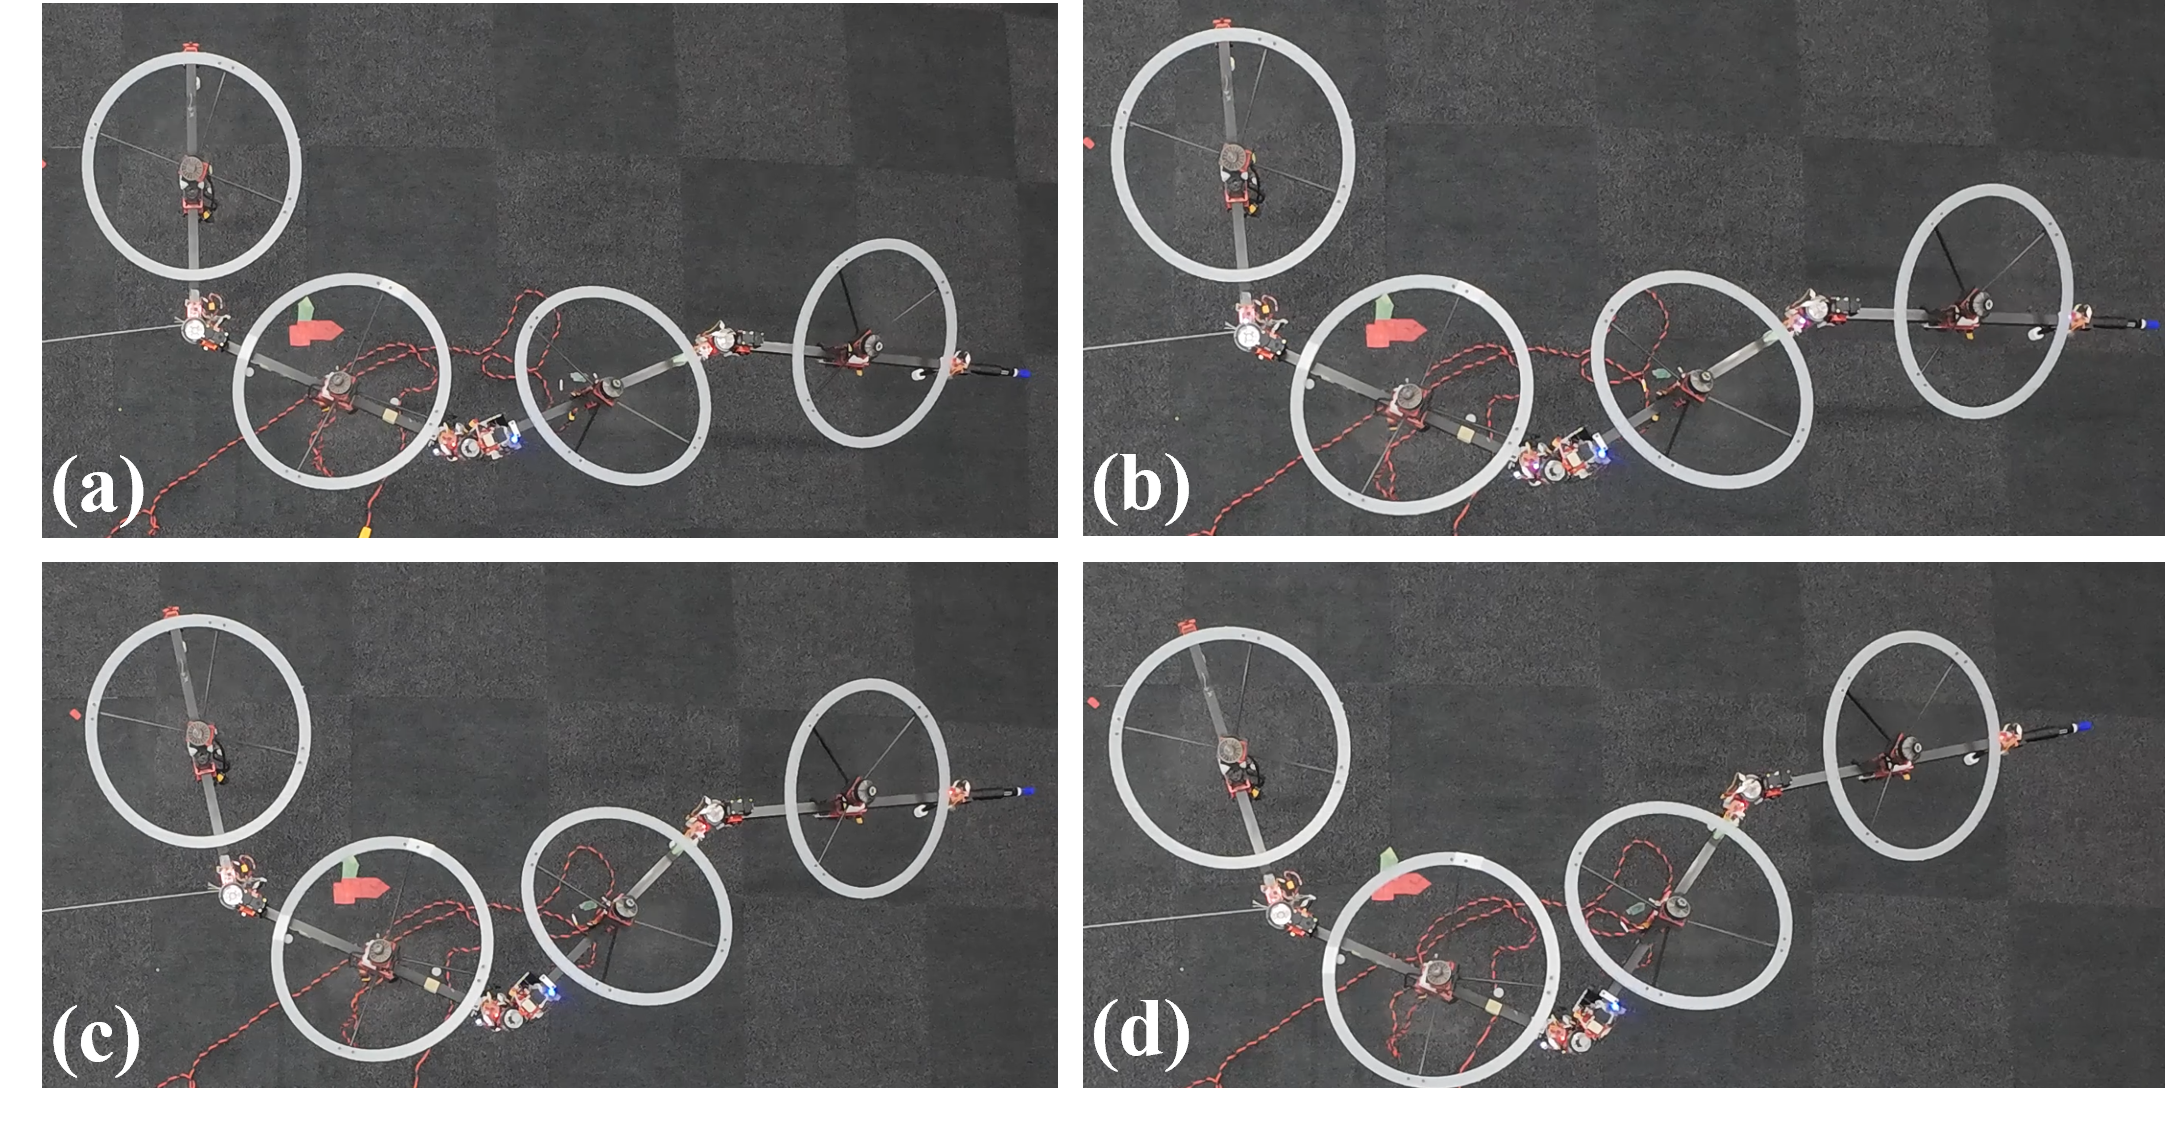
\includegraphics[trim={0cm 0.3cm 0cm 0cm},clip,width=\linewidth]{figures/chapter3/admittance_changing.png}
%     \caption{Admittance changing.}
%     \label{fig:admittance_changing}
%     \vspace{-5mm}
% \end{figure}

% \begin{equation}
% \begin{aligned}
% \min_{\lambda,\,\theta,\,\phi} \quad & \|\boldsymbol{\lambda}\|^2 \\
% \mathrm{s.t.} \quad & ^C\mathbf{w}_{cmd} = \boldsymbol{Q}(\theta,\phi)\boldsymbol{\lambda}
% \end{aligned}
% \end{equation}
% %%%%%%%%%%%%%%%%%%%%%%%%%%%%%%%%%%%%%%%%%%%%%%%%%%%%%%%%%%%%%%%%%%%%%%%%%%%%%%%%



%%%%%%%%%%%%%%%%%%%%%%%%%%%%%%%%%%%%%%%%%%%%%%%%%%%%%%%%%%%%%%%%%%%%%%%%%%%%%%%%
\section{Summary}

In this chapter, we explained how impedance control can modify the dynamic response of the system. We also discussed the difference between the PID controller and impedance controller, focusing on how impedance control can regulate the dynamic response of the system through the desired impedance parameters, especially the mass ratio $\mu$. Finally, the implementation of impedance control for the multi-link aerial robot was presented.